\section{Scientific General Intelligence: Concept and Operational Definition}

Scientific General Intelligence (SGI) refers to an AI system capable of engaging in the full cycle of scientific inquiry with autonomy, versatility, and methodological rigor. Unlike systems that excel at isolated reasoning tasks, an SGI-capable model must integrate knowledge retrieval, idea formation, action execution, and evidence-based interpretation into a coherent, iterative workflow.

To formalize this notion, we characterize scientific cognition through four interdependent stages: \textbf{Deliberation} (evidence search, synthesis, and critical assessment), \textbf{Conception} (generation of hypotheses and ideas), \textbf{Action} (implementation of experiments or simulations), and \textbf{Perception} (interpretation of empirical results). 

Grounded in this framework, we provide an operational definition: an AI system exhibits SGI if it can (1) retrieve, synthesize, and critically evaluate knowledge; (2) generate scientifically grounded and novel ideas; (3) plan and execute experimental procedures; (4) interpret empirical outcomes with causal and contextual awareness.

This definition highlights a central limitation in existing benchmarks~\cite{hendrycks2020measuring, du2025supergpqa, mialon2023gaia, phan2025humanity}: most evaluate factual recall or single-step reasoning, but few examine the structured, long-horizon workflows that constitute real scientific inquiry. 

Building on the operational definition of \textbf{SGI} established in the previous section, we introduce \textit{SGI-Bench} (Scientific Intelligence Benchmark for LLMs via Scientist-Aligned Workflows) — a benchmark designed to empirically evaluate the extent to which large language models (LLMs), vision-language models (VLMs), and agent-based systems exhibit the cognitive and procedural abilities required for scientific discovery. 

SGI-Bench systematically measures AI performance across 10 core scientific domains — astronomy, chemistry, earth science, energy, information science, life science, materials science, neuroscience, physics and math — providing a panoramic view of how AI systems engage with scientific reasoning across disciplines. Its task design draws inspiration from the seminal article \textit{125 Questions: Exploration and Discovery}~\cite{sanders2021125} published in \textit{Science}, ensuring both disciplinary breadth and societal relevance. 


At the heart of SGI-Bench lies the principle of \textit{scientist alignment}—the commitment to evaluating models under conditions that authentically mirror real scientific workflows.
This concept manifests in several ways:
\begin{itemize}
    \item The task designs closely mirror the real-world research scenarios encountered by scientists in their work, ensuring that each task is intrinsically tied to the scientific discovery process.
    \item The raw materials used in task construction are sourced directly from scientists, ensuring the authenticity and relevance of the content.
    \item Scientists have been closely involved in the process of constructing the benchmark, with a \textit{scientist-in-the-loop} approach, ensuring the tasks reflect the nuances of actual scientific workflows.
    \item The final evaluation scores are aligned with the checklist based on the needs of real scientific research scenarios from scientists, which ensures that the assessments genuinely reflect the scientific utility of the models.
\end{itemize}

SGI-Bench departs from conventional benchmarks that emphasize factual recall or single-turn reasoning. Instead, it operationalizes the long-horizon workflow of scientific discovery into four interdependent stages: literature review(Deliberation), methodology design(conception), experiment implementation(Action), and experimental analysis(Perception). These stages correspond to fundamental capabilities required of AI systems: information integration and understanding(Scientific Deep Research), design and planning(Idea Generation), experimental execution(AI-Assisted Scientific Experiment), and reasoning-based interpretation(Scientific Experimental Reasoning). Together, they form a unified framework that measures not only what models know but how they think, plan, and adapt in pursuit of new knowledge. 

\begin{figure}[ht]
% \vspace{-0.5em}
\centerline
{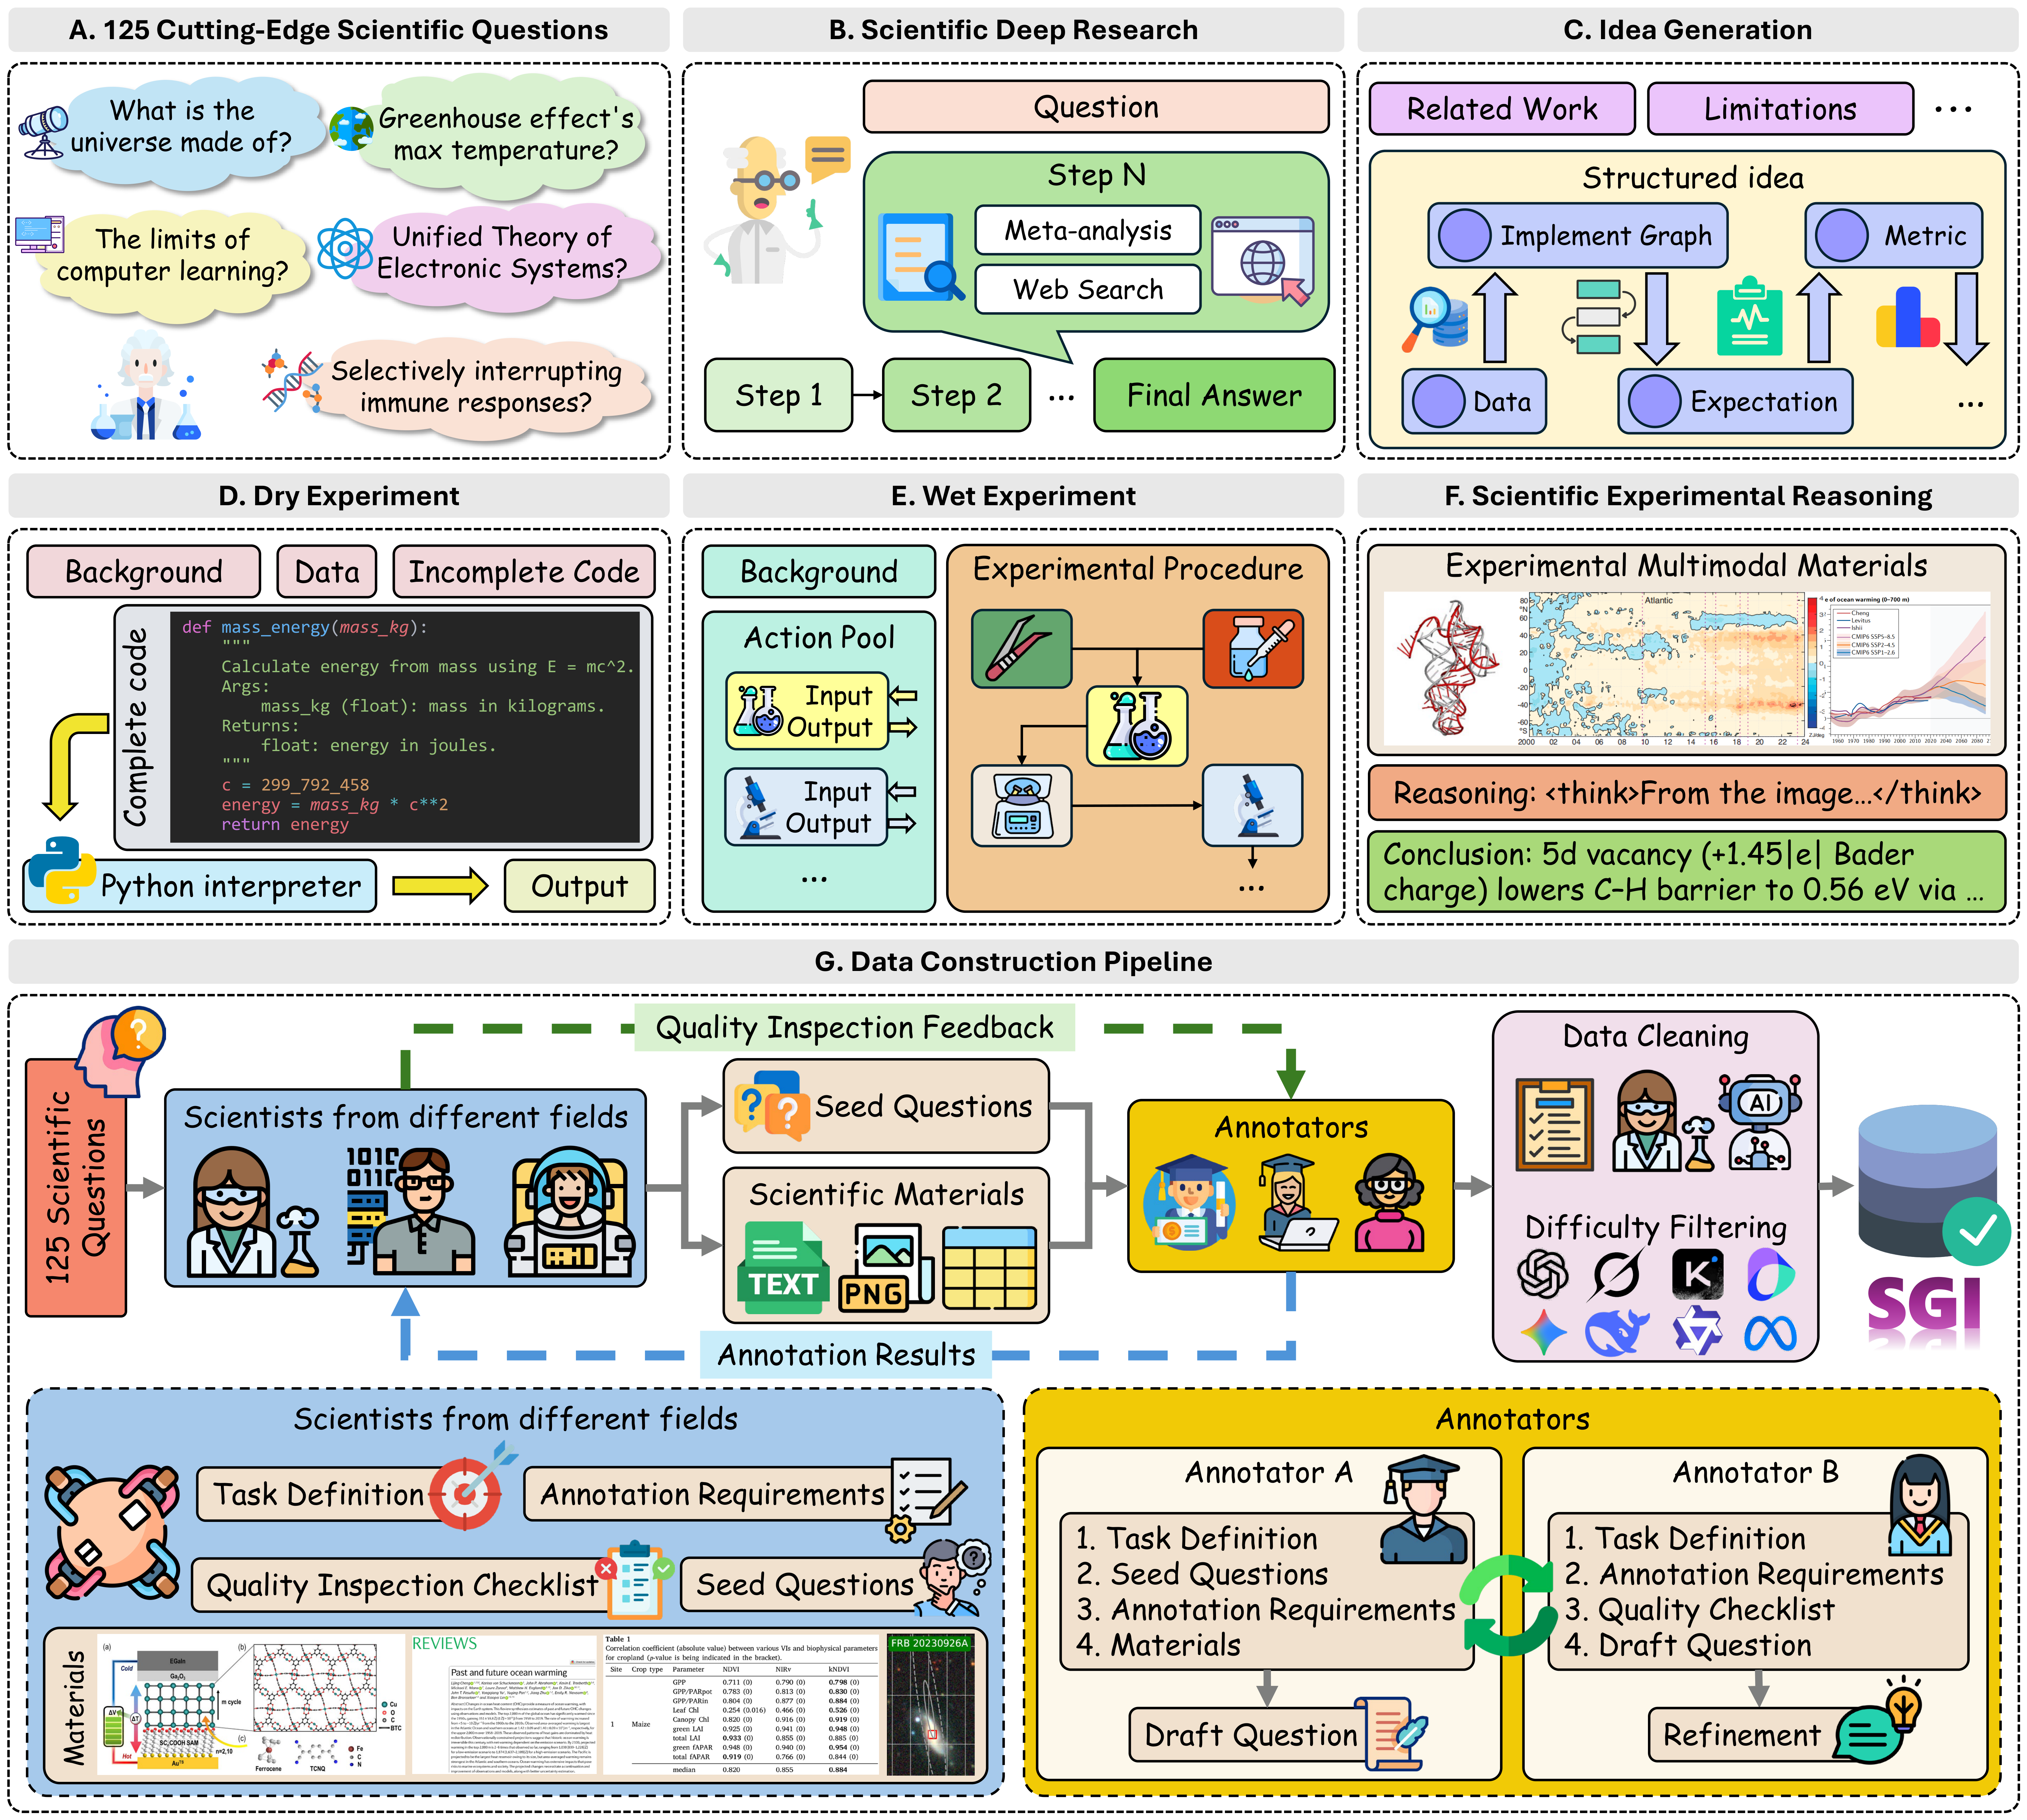
\includegraphics[width=16cm]{paper/imgs/pipeline.png}}
\caption{\textbf{SGI-Bench Workflow Pipeline}: The end-to-end four-stage framework (Deliberation, Conception, Action, Perception) that operationalizes scientific discovery, mapping tasks to capabilities and aligning evaluation with scientist practice.}
\label{fig: pipeline}
% \vspace{-2em}
\end{figure}



\subsection{Task Definition in Scientific Workflow}

\subsubsection{Scientific Deep Research}
Scientific deep research refers to a thorough and comprehensive investigation of a specific scientific topic, combining elements of both AI-driven deep research~\cite{xu2025comprehensive, hu2025flowsearch, shi2025dualresearch} and scientific meta-analysis~\cite{field2010meta, xu2025manalyzer}. This task typically involves multi-step reasoning, web searches, document retrieval, and data analysis. Drawing inspiration from AI’s deep research, which often relies on multi-hop searches to gather diverse information across multiple sources, it also incorporates the methodology of meta-analysis from the scientific community. Meta-analysis, a rigorous form of scientific research, synthesizes existing literature to derive precise, data-driven conclusions and extract quantitative insights from a large body of studies. Unlike general deep research, which may focus on qualitative understanding, meta-analysis centers on aggregating and analyzing data to produce statistically significant results. By combining the multi-hop search nature of AI’s deep research with the systematic, evidence-based approach of meta-analysis, this task ensures results that are both scientifically precise and meaningful. The ability to perform scientific deep research is crucial for advancing scientific knowledge, as it enables AI models to replicate the process of reviewing, synthesizing, and analyzing existing research to formulate new, data-driven hypotheses.

In order to capture the diversity of real-world scientific inquiries, we divide the task of scientific deep research into four representative types: data, properties, micro-experiments, and macro-experiments, as illustrated in Table~\ref{tab:deep_research_types}. This division reflects the major types of questions scientists often confront, ranging from data-centric queries to property characterization, and from small-scale controlled experiments to large-scale natural events. By organizing the task in this way, the benchmark ensures that AI systems are evaluated across the breadth of literature review and data-driven investigation.

\begin{table}[ht]
\centering
\caption{\textbf{Scientific Deep Research Types}: Four representative categories of inquiry targets and their roles in the scientific workflow.}
\label{tab:deep_research_types}
\resizebox{16.0cm}{!}{
\begin{tabular}{p{3.5cm}p{6cm}p{6cm}}
\toprule
\textbf{Type} & \textbf{Core Description} & \textbf{Role in Scientific Workflow} \\
\midrule
\rowcolor{blue!5}Data & Focused on retrieving or analyzing structured datasets, such as event counts, statistical summaries, or dataset-specific attributes. & Supports quantitative literature review and provides a foundation for identifying trends or anomalies. \\
\addlinespace
Property & Concerned with identifying or inferring material, molecular, or system properties, often requiring interpretation of experimental results or theoretical knowledge. & Bridges literature review with methodology design by clarifying key parameters. \\
\addlinespace
\rowcolor{blue!5}Micro-experiment & Small-scale controlled experiments, often involving chemical reactions, physical transformations, or laboratory processes under specific conditions. & Provides simulated reasoning over experimental procedures and outcomes. \\
\addlinespace
Macro-experiment & Large-scale or natural experiments, such as astronomical events, climate observations, or geophysical phenomena. & Extends literature review to global or long-term observations, anchoring hypotheses in real-world contexts. \\
\bottomrule
\end{tabular}
}
\end{table}

In real-world scientific workflows, deep research corresponds to the literature review stage. During this stage, scientists investigate existing studies, gather data, and analyze findings to understand the current state of knowledge and identify knowledge gaps that require further investigation.


\begin{tcolorbox}[
    breakable,
    title=Task Definition of Scientific Deep Research,
    colback=LighterGray,
    colframe=DeepPurple,
    colbacktitle=DeepPurple,
    coltitle=White
]
\textbf{\emph{\textcolor{DeepPurple}{Task Input}}}
\begin{itemize}
    \item \texttt{\textbf{Background (B)}}: A detailed background of the research topic, including the scientific field and subfields, to avoid ambiguities in terminology.
    \item \texttt{\textbf{Constraints (C)}}: Constraints such as experimental settings, scientific assumptions, and data sources that frame the problem appropriately.
    \item \texttt{\textbf{Data (D)}}: Any experimental or empirical data directly mentioned in the task, which might be either explicitly provided or inferred.
    \item \texttt{\textbf{Question (Q)}}: A specific, focused question that the task aims to address, such as determining a particular quantity or its variation over time.
    \item \texttt{\textbf{Response Requirements (R)}}: Specifications for the answer, including the required units and whether the answer should be an integer or a decimal with a specified number of decimal places.
\end{itemize}

\textbf{\emph{\textcolor{DeepPurple}{Task Output}}}
\begin{itemize}
    \item \texttt{\textbf{Steps (S)}}: A detailed, step-by-step approach that the system uses to retrieve and process data or perform reasoning.
    \item \texttt{\textbf{Answer (A)}}: A precise numerical or string-based response, such as a specific value or a phrase.
\end{itemize}

\textbf{\emph{\textcolor{DeepPurple}{Task Formulation}}}
\[
\texttt{S, A} = \texttt{LLM/Agent}(\texttt{B, C, D, Q, R})
\]
\end{tcolorbox}

\begin{figure}[ht]
    \vspace{0.01cm}
    \caption{\textbf{Scientific Deep Research Task}: Inputs, outputs, and formulation for literature-driven quantitative inquiry combining multi-step reasoning and meta-analysis.}
    \label{fig:Task Definition of Scientific Deep Research}
\end{figure}


\subsubsection{Idea Generation}
\label{sec: Idea gen}
Idea generation is a critical component of the scientific process, corresponding to the stage of research methodology design. At this stage, researchers synthesize existing knowledge, engage in associative and creative thinking, and propose new approaches to address current challenges. It embodies the creative essence of scientific inquiry and shapes the direction and potential impact of subsequent research.

In real-world scientific workflows, idea generation typically occurs after researchers have completed a thorough literature review. They integrate prior findings, identify limitations or knowledge gaps, and use creative reasoning to formulate new hypotheses, methods, or frameworks aimed at overcoming these shortcomings. In this sense, idea generation serves as the crucial link between literature understanding and methodological innovation.

However, because idea generation is an open-ended and highly creative task, its evaluation is inherently challenging. To make the assessment more systematic and tractable, we decompose an originally holistic idea into several interrelated components, forming a structured representation of the idea. This decomposition enables more fine-grained evaluation along dimensions such as effectiveness, novelty, level of detail, and feasibility~\cite{moose}.

\begin{tcolorbox}[
    breakable,
    title=Task Definition of Idea Generation,
    colback=LighterGray,
    colframe=DeepPurple,
    colbacktitle=DeepPurple,
    coltitle=White
]
\textbf{\emph{\textcolor{DeepPurple}{Task Input}}}
\begin{itemize}
    \item \texttt{\textbf{Related Work (RW)}}: A summary of existing research relevant to a certain research direction, providing context for new ideas.
    \item \texttt{\textbf{Challenge (C)}}: The current challenges in the field and the limitations of existing solutions.
    \item \texttt{\textbf{Limitation (L)}}: Specific shortcomings or constraints of current research that new ideas need to address.
    \item \texttt{\textbf{Motivation (M)}}: The perspective and motivation of addressing the limitations in this research direction.
    \item \texttt{\textbf{Task Objective (TO)}}: The primary goal of the task, such as generating ideas that solve identified challenges or improve existing solutions.
    \item \texttt{\textbf{Existing Solutions (ES)}}: A description of the current approaches or solutions available in the field.
\end{itemize}

\textbf{\emph{\textcolor{DeepPurple}{Task Output}}}
\begin{itemize}
    \item \texttt{\textbf{Core Idea (CI)}}: The central novel idea or concept generated to address the research challenge.
    \item \texttt{\textbf{Implementation Steps (IS)}}: The steps or procedures required to implement the core idea.
    \item \texttt{\textbf{Implementation Order (IO)}}: The sequence in which the implementation steps should be executed.
    \item \texttt{\textbf{Data (D)}}: The data that will be used to implement the idea or evaluate its effectiveness.
    \item \texttt{\textbf{Evaluation Metrics (EM)}}: The criteria for assessing the success or relevance of the generated idea.
    \item \texttt{\textbf{Expected Outcome (EO)}}: The anticipated result or contribution the idea is expected to achieve.
\end{itemize}

\textbf{\emph{\textcolor{DeepPurple}{Task Formulation}}}
\[
\texttt{CI, IS, IO, D, EM, EO} = \texttt{LLM/Agent}(\texttt{RW, C, L, M, TO, ES})
\]
\end{tcolorbox}

\begin{figure}[ht]
    \vspace{0.01cm}
    \caption{\textbf{Idea Generation Task}: Inputs, outputs, and formulation for methodology design, integrating evaluation metrics and structured implementation planning.}
    \label{fig:Task Definition of Idea Generation}
\end{figure}

\subsubsection{AI-Assisted Scientific Experiment}
\label{sec: Task Definition of Experiment}
Scientific experimentation represents the core of the discovery process, bridging theoretical formulation and empirical validation. Within SGI-Bench, we formalize this process into two complementary categories: \textit{dry} and \textit{wet} experiments. Dry experiments capture computational and simulation-based studies—where AI assists in generating, refining, or executing scientific code that models physical phenomena. Wet experiments, by contrast, simulate laboratory-based workflows, requiring the model to plan and reason about sequences of actions involving physical instruments, reagents, and procedural parameters. Together, these two categories span the continuum from theoretical abstraction to empirical realization, offering a holistic evaluation of how AI can assist scientists in both virtual and physical experimentation.

\paragraph{Dry Experiment}
Dry experiments emphasize computational problem-solving, reflecting the growing role of AI in automating simulation-driven science. Each task presents the model with incomplete or masked scientific code that encapsulates domain-specific computations, such as molecular dynamics, climate modeling, or numerical solvers in physics. The model must infer the missing logic, reconstruct executable code, and ensure that the resulting program produces correct and efficient outcomes. This task thus evaluates a model’s ability to integrate scientific understanding with code synthesis—testing not only syntactic correctness but also conceptual fidelity to the underlying scientific problem.

To better characterize the scope of dry experiments, we categorize representative computational functions commonly encountered across disciplines, including numerical calculation, statistical analysis, simulation, metric calculation, data processing, and predictive modeling, as shown in Table~\ref{tab:dry_experiment_functions}. The completion or generation of these functions offers a rigorous measure of how well AI systems can operationalize scientific intent into executable form.

\begin{table}[ht]
\centering
\caption{\textbf{Dry Experiment Function Types}: Representative computational functions and their roles across scientific code-completion tasks.}
\label{tab:dry_experiment_functions}
\resizebox{15.5cm}{!}{
\begin{tabular}{p{5cm}p{10cm}}
\toprule
\textbf{Function Category} & \textbf{Core Role in Scientific Experiments} \\
\midrule
\rowcolor{blue!5}Numerical Calculation & Basic mathematical computations required to support physical or chemical modeling. \\
\addlinespace
Statistical Analysis & Processing experimental data using descriptive or inferential statistics to identify trends and distributions. \\
\addlinespace
\rowcolor{blue!5}Simulation & Running computational simulations (e.g., molecular dynamics, finite element analysis) and filtering results for relevant conditions. \\
\addlinespace
Metric Calculation & Computing evaluation metrics such as accuracy, error, or performance indicators for validating experiments. \\
\addlinespace
\rowcolor{blue!5}Data Processing & Handling raw data before and after experiments, including normalization, cleaning, and feature extraction. \\
\addlinespace
Predictive Modeling & Applying machine learning methods to categorize, predict, or group experimental results. \\
\bottomrule
\end{tabular}
}
\end{table}


In real scientific workflows, dry experiments correspond to the stage of experimental design in computational and simulation-based studies. Following hypothesis formulation, researchers employ virtual experiments to anticipate and evaluate potential outcomes prior to empirical validation, enabling a cost-efficient and theoretically grounded pre-assessment of experimental feasibility.

\begin{tcolorbox}[
    breakable,
    title=Task Definition of Dry Experiment,
    colback=LighterGray,
    colframe=DeepPurple,
    colbacktitle=DeepPurple,
    coltitle=White
]
\textbf{\emph{\textcolor{DeepPurple}{Task Input}}}
\begin{itemize}
    \item \texttt{\textbf{Background (B)}}: Information from relevant scientific code, providing context for the dry experiment.
    \item \texttt{\textbf{Data Code (D)}}: The data used in the experiment, including any code snippets or predefined inputs.
    \item \texttt{\textbf{Main Code (M)}}: The core experimental code where some functions may be masked or missing.
\end{itemize}

\textbf{\emph{\textcolor{DeepPurple}{Task Output}}}
\begin{itemize}
    \item \texttt{\textbf{Functions (F)}}: The missing functions in the main code \( M \), which the system is tasked with generating or completing.
\end{itemize}

\textbf{\emph{\textcolor{DeepPurple}{Task Formulation}}}
\[
\texttt{F} = \texttt{LLM/Agent}(\texttt{B, D, M})
\]
\end{tcolorbox}

\begin{figure}[ht]
    \vspace{0.01cm}
    \caption{\textbf{Dry Experiment Task}: Inputs, outputs, and formulation for code-completion based computational studies with masked functions.}
    \label{fig:Task Definition of Dry Experiment}
\end{figure}

\paragraph{Wet Experiment}
Wet experiments represent the physical realization of scientific inquiry, encompassing laboratory and field-based procedures that transform theoretical designs into empirical evidence. These tasks simulate the execution phase of real-world experiments, where models are required to plan, organize, and reason through sequences of atomic actions involving materials, instruments, and procedural parameters. Given inputs describing experimental objectives, configurations, and available tools, the model must generate structured, executable protocols that are both accurate and practically feasible. Evaluation considers not only the correctness of individual steps but also their procedural coherence and alignment with established laboratory conventions.

In real scientific workflows, wet experiments correspond to the execution and validation stages of discovery. This is where hypotheses are tested against the physical world, data are collected, and evidence is generated to confirm, refine, or refute prior assumptions. By assessing how effectively AI systems can design and reason through these embodied experimental processes, this task provides a window into their capacity to bridge symbolic understanding with real-world scientific practice.

\begin{tcolorbox}[
    breakable,
    title=Task Definition of Wet Experiment,
    colback=LighterGray,
    colframe=DeepPurple,
    colbacktitle=DeepPurple,
    coltitle=White
]
\textbf{\emph{\textcolor{DeepPurple}{Task Input}}}
\begin{itemize}
    \item \texttt{\textbf{Background (B)}}: Information from relevant experimental procedure.
    \item \texttt{\textbf{Action Pool (AP)}}: A predefined set of atomic actions that can be used in the experiment, along with explanations and corresponding input/output definitions.
\end{itemize}

\textbf{\emph{\textcolor{DeepPurple}{Task Output}}}
\begin{itemize}
    \item \texttt{\textbf{Atomic Action Order (AAO)}}: The order in which atomic actions should be executed.
    \item \texttt{\textbf{Atomic Action Parameters (AAP)}}: The parameters associated with each atomic action (e.g., reagents, temperature).
\end{itemize}

\textbf{\emph{\textcolor{DeepPurple}{Task Formulation}}}
\[
\texttt{AAO, AAP}= \texttt{LLM/Agent}(\texttt{B, AP})
\]
\end{tcolorbox}

\begin{figure}[ht]
    \vspace{0.01cm}
    \caption{\textbf{Wet Experiment Task}: Inputs, outputs, and formulation for laboratory protocol planning via atomic actions and parameters.}
    \label{fig:Task Definition of Wet Experiment}
\end{figure}

\subsubsection{Scientific Experimental Reasoning}

Scientific experimental reasoning in this benchmark focuses on multi-modal scientific reasoning, requiring models to interpret heterogeneous information drawn from diverse sources~\cite{zhang2024cmmmuchinesemassivemultidiscipline}. We consider five representative modalities as shown in Table~\ref{tab:modalities}: a) process images that integrate symbolic and textual information to depict workflows or variable relationships; b) observation images representing raw data captured by instruments such as telescopes, satellites, or microscopes; c) experiment images documenting laboratory setups and procedures; d) simulation images generated by computational models to visualize physical or chemical processes; and e) visualization images such as plots or charts that reveal patterns within structured datasets. Collectively, these modalities reflect the multi-faceted and evidence-driven nature of scientific inquiry.

\begin{table}[ht]
\centering
\caption{\textbf{Scientific Experimental Reasoning Modalities}: Five visual modalities used for multi-modal evidence and analysis.}
\label{tab:modalities}
\resizebox{16.0cm}{!}{
\begin{tabular}{p{4cm}p{6cm}p{6cm}}
\toprule
\textbf{Modality} & \textbf{Core Description} & \textbf{Scientific Role} \\
\midrule
\rowcolor{blue!5}Process Images & Graphical symbols + text describing workflows or variable relations. & Capture the logical flow of experiments and research design. \\
\addlinespace
Observation Images & Raw data from instruments (e.g., telescope, satellite, microscope). & Provide direct evidence of natural or physical phenomena. \\
\addlinespace
\rowcolor{blue!5}Experiment Images & Photos of instruments, setups, or lab operations. & Document experimental configurations and operational details. \\
\addlinespace
Simulation Images & Generated from computational models/software. & Visualize theoretical predictions of physical or chemical processes. \\
\addlinespace
\rowcolor{blue!5}Visualization Images & Processed structured data into charts/plots. & Reveal patterns, comparisons, or correlations from datasets. \\
\bottomrule
\end{tabular}
}
\end{table}

To reason effectively over such diverse inputs, we define four complementary reasoning paradigms as shown in Table~\ref{tab:reasoning_paradigms}: a) signal perception, focusing on the extraction of direct patterns from visual signals; b) attribute understanding, which demands domain knowledge to interpret key visual or contextual features; c) comparative reasoning, involving integration and comparison across multiple sources to ensure consistency and rigor; and d) causal reasoning, aimed at uncovering underlying mechanisms and scientific principles. These paradigms collectively span the hierarchy from low-level perception to high-level scientific inference.

\begin{table}[ht]
\centering
\caption{\textbf{Scientific Experimental Reasoning Paradigms}: Four reasoning paradigms spanning perception to causality with examples and requirements.}
\label{tab:reasoning_paradigms}
\resizebox{16.0cm}{!}{
\begin{tabular}{p{4cm}p{6cm}p{6cm}}
\toprule
\textbf{Reasoning Paradigm} & \textbf{Core Requirement} & \textbf{Typical Example} \\
\midrule
\rowcolor{blue!5}Signal Perception & Direct extraction of information from visual signals without heavy prior knowledge. & Identifying patterns in telescope images or microscope slides. \\
\addlinespace
Attribute Understanding & Requires disciplinary background to interpret key features and scientific attributes. & Recognizing crystalline structures in materials science images. \\
\addlinespace
\rowcolor{blue!5}Comparative Reasoning & Integrates and contrasts information across multiple images, often cross-domain. & Comparing climate model simulations with satellite observations. \\
\addlinespace
Causal Reasoning & Goes beyond correlation to infer mechanisms or propose hypotheses. & Inferring causal pathways in gene expression from multi-modal experimental data. \\
\bottomrule
\end{tabular}
}
\end{table}

In real-world scientific workflows, experimental reasoning corresponds to the data analysis stage, during which scientists interpret experimental and simulated data, perform comparative analyses, and refine hypotheses based on empirical evidence.

\begin{tcolorbox}[
    breakable,
    title=Task Definition of Scientific Experimental Reasoning,
    colback=LighterGray,
    colframe=DeepPurple,
    colbacktitle=DeepPurple,
    coltitle=White
]
\textbf{\emph{\textcolor{DeepPurple}{Task Input}}}
\begin{itemize}
    \item \texttt{\textbf{Multiple Experimental Images (MEI)}}: A set of images representing various experimental outcomes or data collected from instruments.
    \item \texttt{\textbf{Question (Q)}}: A specific question or hypothesis related to the experimental data that requires reasoning or analysis.
\end{itemize}

\textbf{\emph{\textcolor{DeepPurple}{Task Output}}}
\begin{itemize}
    \item \texttt{\textbf{Reasoning (R)}}: The specific steps in the reasoning process, including calculation, thinking, analysis, etc..
    \item \texttt{\textbf{Answer (A)}}: The conclusion drawn from analyzing the experimental data, answering the specified question or hypothesis.
\end{itemize}

\textbf{\emph{\textcolor{DeepPurple}{Task Formulation}}}
\[
\texttt{R, A} = \texttt{LLM/Agent}(\texttt{MEI, Q})
\]
\end{tcolorbox}

\begin{figure}[ht]
    \vspace{0.01cm}
    \caption{\textbf{Scientific Experimental Reasoning Task}: Inputs, outputs, and formulation for multi-modal analysis with step-by-step reasoning and final answers.}
    \label{fig:Task Definition of Scientific Experimental Reasoning}
\end{figure}


\subsection{Multi-Dimensional Metrics}
\label{sec:Metrics}

To align with the scientific characteristics of each task, we have designed multi-dimensional evaluation metrics for every task. This approach avoids a one-size-fits-all binary judgment and instead provides a more fine-grained assessment.

\subsubsection{Metrics of Scientific Deep Research}

The Scientific Deep Research task draws inspiration from AI’s deep research paradigms~\cite{wenxiaobai,DeepResearch_OpenAI2025,Perplexity_DeepResearch_2025,KimiResearcher_2025,GrokDeepSearch_2025} while incorporating methodologies from meta-analysis in the scientific domain. The former emphasizes multi-step reasoning, where solving a problem often requires iterative searches, calculations, and inferences; the correctness of each step directly impacts the accuracy of the final answer. The latter focuses on systematically extracting and synthesizing data from literature, requiring highly precise results. Accordingly, our metrics capture both step-by-step reasoning fidelity and final answer accuracy.

\begin{tcolorbox}[
    breakable,
    title=Metric Definition of Exact Match,
    colback=LighterGray,
    colframe=DeepPurple,
    colbacktitle=DeepPurple,
    coltitle=White
]
\textbf{Exact Match (EM)}: Since the Scientific Deep Research tasks are designed to have short, unique, and easily verifiable answers, we use exact match as a hard metric to assess whether the model’s final answer is correct. The model receives a score of 1 if the output exactly matches the reference answer, and 0 otherwise.
\end{tcolorbox}

\begin{tcolorbox}[
    breakable,
    title=Metric Definition of Step-Level Accuracy,
    colback=LighterGray,
    colframe=DeepPurple,
    colbacktitle=DeepPurple,
    coltitle=White
]
\textbf{Step-Level Accuracy (SLA)}: Models are required to produce step-by-step solutions. We employ an LLM-based judge to compare each model-generated step against the reference solution steps. For each step, the judge determines whether it is correct and provides reasoning. This fine-grained evaluation avoids binary correctness judgments for the entire solution, allowing precise assessment of reasoning accuracy at each inference step. The metric is computed as the proportion of steps correctly solved relative to the total number of steps. The score is calculated as
\[
\text{SLA} = \frac{\text{Number of correct reasoning steps}}{\text{Total number of reasoning steps}}.
\]

\end{tcolorbox}



\subsubsection{Metrics of Idea Generation}
\label{Metrics: Idea Gen}

To evaluate the open-ended nature of idea generation, we adopt a hybrid framework that integrates both subjective and objective metrics. We assess each idea along four dimensions---\textbf{effectiveness}, \textbf{novelty}, \textbf{detailedness}, and \textbf{feasibility}---which together characterize an idea's scientific quality, creativity, and executability~\cite{moose,ruan2025liveideabenchevaluatingllmsdivergent}.

\textbf{Subjective Evaluation via LLM Judges.}
For subjective scoring, we perform pairwise comparisons between model-generated ideas and expert-written reference ideas. For each of the four dimensions, an LLM judge selects which idea is superior. To ensure fairness and robustness, we employ three different LLM judges, each casting two independent votes, resulting in a total of six votes per dimension. The pairwise win rate against the reference idea is then used as the subjective component of the score for each dimension.

\textbf{Objective Evaluation via Computable Metrics.}
In addition to subjective judgments, we design dimension-specific computational metrics that capture structured properties of the ideas.

\begin{tcolorbox}[
    breakable,
    title=Metric Definition of Effectiveness,
    colback=LighterGray,
    colframe=DeepPurple,
    colbacktitle=DeepPurple,
    coltitle=White
]

For each reference idea, human experts extract its 3--5 most essential keywords. We compute the hit rate of these keywords in the model-generated idea, allowing semantic matches to avoid underestimating effectiveness. The final effectiveness score is the average of the keyword hit rate and the LLM-judge win rate:
\[
\text{Effectiveness} = \frac{\text{Keyword Hit Rate} + \text{LLM Win Rate}}{2}.
\]


\end{tcolorbox}


\begin{tcolorbox}[
    breakable,
    title=Metric Definition of Novelty,
    colback=LighterGray,
    colframe=DeepPurple,
    colbacktitle=DeepPurple,
    coltitle=White
]
We measure novelty by computing the dissimilarity between the model-generated idea and prior related work. Lower similarity indicates that the model proposes ideas not present in existing literature and therefore exhibits higher creativity. The final novelty score averages the dissimilarity score and the subjective win rate:
\[
\text{Novelty} = \frac{\text{Dissimilarity Score} + \text{LLM Win Rate}}{2}.
\]

\end{tcolorbox}


\begin{tcolorbox}[
    breakable,
    title=Metric Definition of Detailedness,
    colback=LighterGray,
    colframe=DeepPurple,
    colbacktitle=DeepPurple,
    coltitle=White
]

We evaluate detailedness from two angles: a) content completeness, which checks whether the idea contains required components (Core Idea, Implementation Steps, Implementation Order, Dataset, Evaluation Metrics, Expected Outcome), and b) redundancy penalty, computed via sentence-level semantic similarity. Ideas with many repetitive sentences are penalized, as verbosity without substance does not constitute genuine detail. The final detailedness score is:
\[
\text{Detailedness} = \frac{\text{Completeness Score (with Penalty)} + \text{LLM Win Rate}}{2}.
\]

\end{tcolorbox}


\begin{tcolorbox}[
    breakable,
    title=Metric Definition of Feasibility,
    colback=LighterGray,
    colframe=DeepPurple,
    colbacktitle=DeepPurple,
    coltitle=White
]

For each research direction, domain experts provide a standardized \textit{implementation graph} containing the essential nodes and their execution order. We extract an implementation graph from each model-generated idea and compute its similarity to the expert template. A low similarity indicates that the proposed idea does not align with accepted solution workflows and is therefore infeasible. The final feasibility score is:
\[
\text{Feasibility} = \frac{\text{Graph Similarity} + \text{LLM Win Rate}}{2}.
\]

\end{tcolorbox}

Taken together, the hybrid subjective--objective design provides a robust, interpretable, and comprehensive assessment of LLMs' scientific idea generation capabilities across creativity, structural clarity, and practical executability.

\subsubsection{Metrics of AI-Assisted Scientific Experiment}

\paragraph{Dry Experiment}
\label{sec: Metric of Dry Experiment}
Dry experiments focus on code generation task. Specifically, each problem includes background information, data code, and main code with certain functions masked. The model is tasked with completing the missing functions. Each problem contains 5 unit tests. Our metrics capture both correctness and execution behavior of the generated code.~\cite{jain2024livecodebenchholisticcontaminationfree}

\begin{tcolorbox}[
    breakable,
    title=Metric Definition of Pass All k Unit Tests,
    colback=LighterGray,
    colframe=DeepPurple,
    colbacktitle=DeepPurple,
    coltitle=White
]
\textbf{Pass all k Unit Tests(PassAll@k)}: This metric measures the proportion of problems with k or more unit tests passed successfully. It’s important to distinguish this from Pass@k. While Pass@k requires only one successful attempt out of k trials, PassAll@k demands that at least k attempts pass the unit tests. Consequently, PassAll@5 represents the most challenging criterion. The score is calculated as
\[
\text{PassAll@k} = \frac{\text{Number of problems with k or more unit tests passed}}{\text{Total number of problems}}.
\]
\end{tcolorbox}

\begin{tcolorbox}[
    breakable,
    title=Metric Definition of Average Execution Time,
    colback=LighterGray,
    colframe=DeepPurple,
    colbacktitle=DeepPurple,
    coltitle=White
]
\textbf{Average Execution Time (AET)}: This metric captures the efficiency of the generated code by measuring the average runtime across all test cases:
\[
\text{AET} = \frac{1}{N} \sum_{i=1}^{N} t_i,
\]
where \(t_i\) is the execution time of the \(i\)-th test case and \(N\) is the total number of test cases.
\end{tcolorbox}

\begin{tcolorbox}[
    breakable,
    title=Metric Definition of Smooth Execution Rate,
    colback=LighterGray,
    colframe=DeepPurple,
    colbacktitle=DeepPurple,
    coltitle=White
]
\textbf{Smooth Execution Rate (SER)}: This metric measures the proportion of generated code that runs without any runtime errors, regardless of correctness of output. It reflects adherence to basic coding standards and robustness:
\[
\text{SER} = \frac{\text{Number of code executions without errors}}{\text{Total number of code executions}}.
\]
\end{tcolorbox}

\paragraph{Wet Experiment}

Wet experiments involve procedural steps using laboratory instruments. Correct execution requires both the correct sequence of actions and proper parameter settings. Accordingly, we propose the following metrics:

\begin{tcolorbox}[
    breakable,
    title=Metric Definition of Sequence Similarity,
    colback=LighterGray,
    colframe=DeepPurple,
    colbacktitle=DeepPurple,
    coltitle=White
]
\textbf{Sequence Similarity (SS)}: This metric evaluates the similarity between the order of atomic actions provided by the model and the reference sequence. Let \(\text{seq}_\text{model}\) and \(\text{seq}_\text{ref}\) be the sequences of atomic actions from the model and the reference, respectively. Denote by \(\text{Inv}(\text{seq}_\text{model}, \text{seq}_\text{ref})\) the number of discordant pairs between the sequences. For sequences of length \(n\), the score is computed as:
\[
\text{SS} = 1 - \frac{\text{Inv}(\text{seq}_\text{model}, \text{seq}_\text{ref})}{\frac{n(n-1)}{2}},
\]
where \(\frac{n(n-1)}{2}\) is the maximum possible number of inversions. By definition, \(\text{SS} = 1\) indicates that the sequences are identical, while \(\text{SS} = 0\) indicates maximal disorder relative to the reference sequence.
\end{tcolorbox}


\begin{tcolorbox}[
    breakable,
    title=Metric Definition of Parameter Accuracy,
    colback=LighterGray,
    colframe=DeepPurple,
    colbacktitle=DeepPurple,
    coltitle=White
]
\textbf{Parameter Accuracy (PA)}: This metric measures the correctness of input parameters for each atomic action compared to the reference, including reagent types, concentrations, volumes, or other domain-specific parameters. The score is calculated as the proportion of correctly specified parameters across all actions:
\[
\text{PA} = \frac{\text{Number of correctly specified parameters}}{\text{Total number of parameters}}.
\]
\end{tcolorbox}



\subsubsection{Metrics of Scientific Experimental Reasoning}
The Scientific Experimental Reasoning task assesses the multi-modal scientific reasoning capabilities of LLMs and agents. 
Specifically, given several images and a corresponding question, the model is required to select the correct option from no fewer than 10 candidates. 
For evaluation, the correctness of the final answer and the validity of intermediate reasoning are equally critical. 
Therefore, two evaluation metrics are adopted, as detailed below.

\begin{tcolorbox}[
    breakable,
    title=Metric Definition of MCA,
    colback=LighterGray,
    colframe=DeepPurple,
    colbacktitle=DeepPurple,
    coltitle=White
]
\textbf{Multi-choice Accuracy (MCA)}: Given several options, the model receives a score of 1 if the selected option exactly matches the reference answer, and 0 otherwise.
The final score of MCA is the average of all individual scores across all test samples. 
This metric directly quantifies the model’s ability to pinpoint the correct solution from a large candidate pool, serving as a foundational measure of its end-to-end scientific reasoning accuracy in the multi-modal task.
\end{tcolorbox}

\begin{tcolorbox}[
    breakable,
    title=Metric Definition of Reasoning Validity,
    colback=LighterGray,
    colframe=DeepPurple,
    colbacktitle=DeepPurple,
    coltitle=White
]
\textbf{Reasoning Validity (RV)}: 
Models are required to generate step-by-step logical reasoning to justify their selected answers. 
An LLM-based judge is utilized to assess the model-generated reasoning against a reference reasoning. 
For each test sample, the LLM judge assigns a validity score ranging from 0 (completely invalid, contradictory, or irrelevant) to 10 (fully rigorous, logically coherent, and perfectly aligned with the reference reasoning), accompanied by justifications for the assigned score. 
This fine-grained scoring paradigm circumvents the limitations of binary correctness assessments, enabling precise quantification of reasoning quality, including the validity of premises, logical transitions, and alignment with scientific principles. 
The final RV score is computed as the mean of individual sample scores across the entire test set, reflecting the model’s overall capability to perform interpretable and reliable scientific reasoning.
\end{tcolorbox}


\subsection{Scientist-Aligned Data Construction}

\paragraph{Raw Corpus Collection}  
In this stage, we conducted multiple discussions with experts from diverse scientific disciplines, drawing from both the 125 important scientific questions published in \textit{Science}, and the prominent research directions in various disciplines with significant scientific impact. Ultimately, we curated 75 research directions spanning ten scientific domains, as shown in Figure~\ref{fig: subjects}. Please refer to Appendix~\ref{sec: all disciplines} for a complete list of research directions.

Subsequently, we collected raw data provided by experts and researchers, primarily consisting of scientific texts and images across the various disciplines. The texts mainly cover knowledge introduction, methodological design, experimental procedures, and data analysis. The images include experiment figures, data visualizations, and observational images, each accompanied by detailed descriptions.

In addition, these experts and researchers will provide seed questions and annotation requirements for annotation, which provide initial examples for the subsequent annotation process, as illustrated in Figure~\ref{fig: pipeline} (G).

\paragraph{Question Construction}  
After gathering the raw data, we recruited over 100 graduate students and PhD candidates from different disciplines to construct benchmark questions according to the task definitions. Annotators first analyzed the collected texts and images, and then created questions according to annotation requirements and seed questions. Several rules were applied to ensure scientific validity and authenticity. Specifically, annotators were required to reference the original data source and paragraph for each question, ensuring traceability to scientist-provided data. Furthermore, all questions are constructed by at least two annotators, one of whom is responsible for generating complex draft questions, and the other is responsible for refining them, as shown in Figure~\ref{fig: pipeline} (G).

During question construction, experts continuously reviewed the generated questions. Each question was immediately submitted to the relevant expert for evaluation, who assessed its scientific value. For instance, a question with an experiment configuration that lacks general applicability would be deemed scientifically invalid. Experts provided feedback to annotators, who then revised the questions accordingly, ensuring that the constructed questions remain aligned with the perspectives and standards of domain scientists.

\paragraph{Data Cleaning}  
Once all questions were constructed, we applied three layers of data cleaning:  
1. \textit{Rule-based cleaning}: Questions that did not meet task-specific criteria were removed. For example, for Scientific Deep Research, steps must be short sentences forming a list, each representing one step; for Wet Experiments, each action must exist in the predefined action pool.  
2. \textit{Model-based cleaning}: Large language models were used to detect and remove questions with semantic errors or potential logical inconsistencies.  
3. \textit{Expert quality check}: All questions were reviewed by the original data-providing scientists, removing incomplete questions, questions with non-unique answers, or questions whose research direction did not align with the source data. For Dry Experiments, Python environments were used to test all code snippets to ensure executability.

\paragraph{Difficulty Filtering}  
After data cleaning, we filtered questions based on difficulty using mainstream LLMs. We evaluated each question with six high-performance models (e.g., GPT-5~\cite{GPT5_SystemCard2025}, Gemini-2.5-Pro~\cite{comanici2025gemini}, DeepSeek-R1~\cite{Guo2025}, Kimi-k2~\cite{team2025kimi}) under a setup allowing web search and deep-reasoning modes. Questions that more than half of the models could correctly answer were removed. This process ensures that the benchmark remains highly challenging.

Through these four steps, we guarantee that all benchmark questions are derived from authentic scientific data, aligned with domain scientists’ judgment of scientific value, and maintain both high quality and high challenge.



\subsection{Data Distribution}

\begin{figure}[ht]
% \vspace{-0.5em}
\centerline
{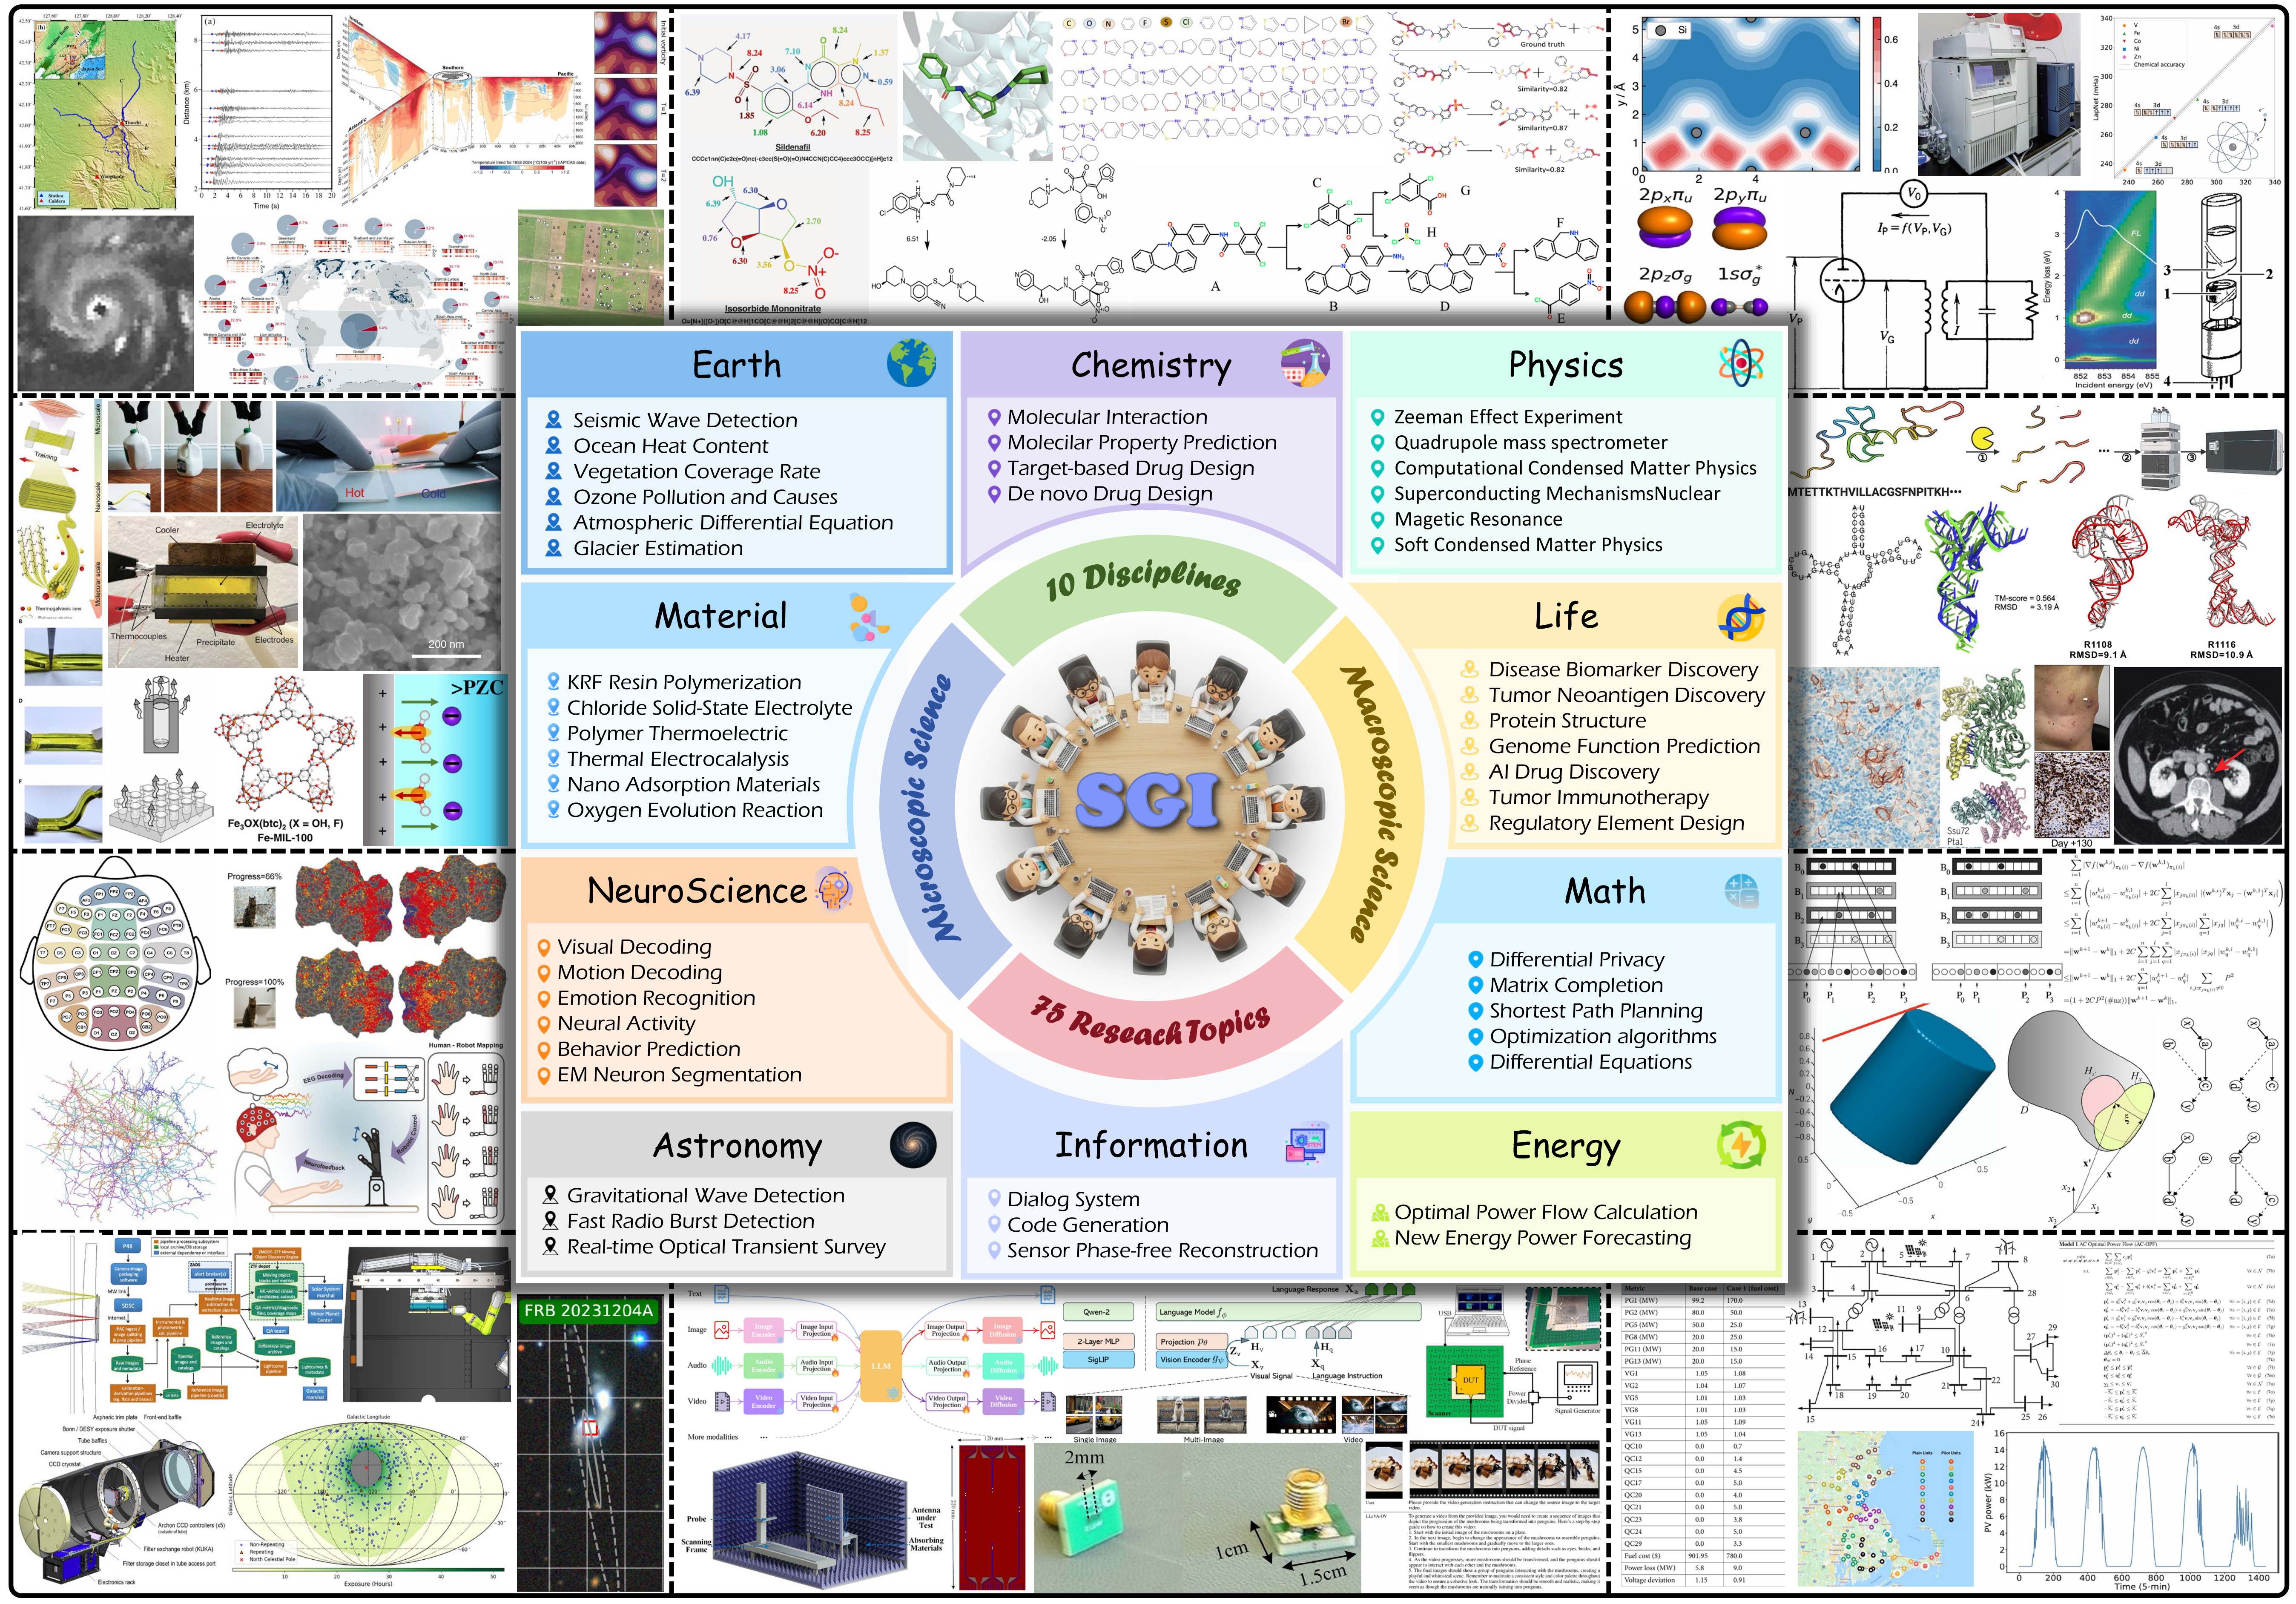
\includegraphics[width=16cm]{paper/imgs/subjects.png}}
% {\includegraphics[width=16cm]{paper/imgs/subjects_v2.png}}
\caption{\textbf{Benchmark Subjects}: Overview of 10 scientific domains covered by SGI-Bench.}
\label{fig: subjects}
% \vspace{-2em}
\end{figure}

After the data construction process, we obtained the complete SGI-Bench benchmark, which contains 318 Scientific Deep Research questions, 315 Idea Generation questions, 271 AI-Assisted Scientific Dry Experiment questions, 68 Wet Experiment questions, and 291 Scientific Experimental Reasoning questions. The discipline distributions for Scientific Deep Research, Idea Generation, and Scientific Experimental Reasoning are identical, as shown in Figure~\ref{fig: data_distribution} (a). The discipline distributions for Dry and Wet Experiments are presented in Figure~\ref{fig: data_distribution} (b) and Figure~\ref{fig: data_distribution} (c), respectively, with Wet Experiments covering only a subset of disciplines, such as Biology and Chemistry.

\begin{figure}[ht]
% \vspace{-0.5em}
\centerline
{\includegraphics[width=15cm]{paper/imgs/data_distribution.png}}
\caption{\textbf{Benchmark Data Distribution}: (a) Overall discipline distribution; (b) Dry experiment discipline distribution; (c) Wet experiment discipline distribution; (d) Scientific Deep Research question types; (e) Dry Experiment function types; (f) Scientific Experimental Reasoning image modalities; (g) Scientific Experimental Reasoning reasoning paradigms.}
\label{fig: data_distribution}
% \vspace{-2em}
\end{figure}

In addition to discipline-level distributions, we further categorized the tasks at a finer granularity. For Scientific Deep Research, questions are grouped based on the type of target being investigated into four categories: Data, Properties, Micro-Experiments, and Macro-Experiments, as detailed in Table~\ref{tab:deep_research_types}. The distribution of these types is illustrated in Figure~\ref{fig: data_distribution} (d). For Dry Experiments, questions are classified into six types according to the masked function type, as shown in Table~\ref{tab:dry_experiment_functions}, with the corresponding distribution displayed in Figure~\ref{fig: data_distribution} (e). In Scientific Experimental Reasoning, the task inputs include images spanning multiple modalities, including Process Images, Observation Images, Experiment Images, Simulation Images, and Visualization Images, summarized in Table~\ref{tab:modalities} and visualized in Figure~\ref{fig: data_distribution} (f). Moreover, based on the type of reasoning required, questions are further categorized into Signal Perception, Attribute Understanding, Comparative Reasoning, and Causal Reasoning, as detailed in Table~\ref{tab:reasoning_paradigms}, with distributions shown in Figure~\ref{fig: data_distribution} (g).

These fine-grained categorizations by discipline and task type facilitate a detailed analysis of the limitations of evaluated LLMs and agents across scientific domains and research tasks. Such insights provide clear directions for advancing AI-assisted scientific discovery.
